% FIG ch07-07 battery common errors overlay (Chinese)
\definecolor{ch07err}{HTML}{C0392B}
\definecolor{ch07Li}{HTML}{D9822B}
\definecolor{ch07wire}{HTML}{3A3A3A}
\begin{tikzpicture}
  \node[anchor=south west, inner sep=0] (img) at (0,0)
    {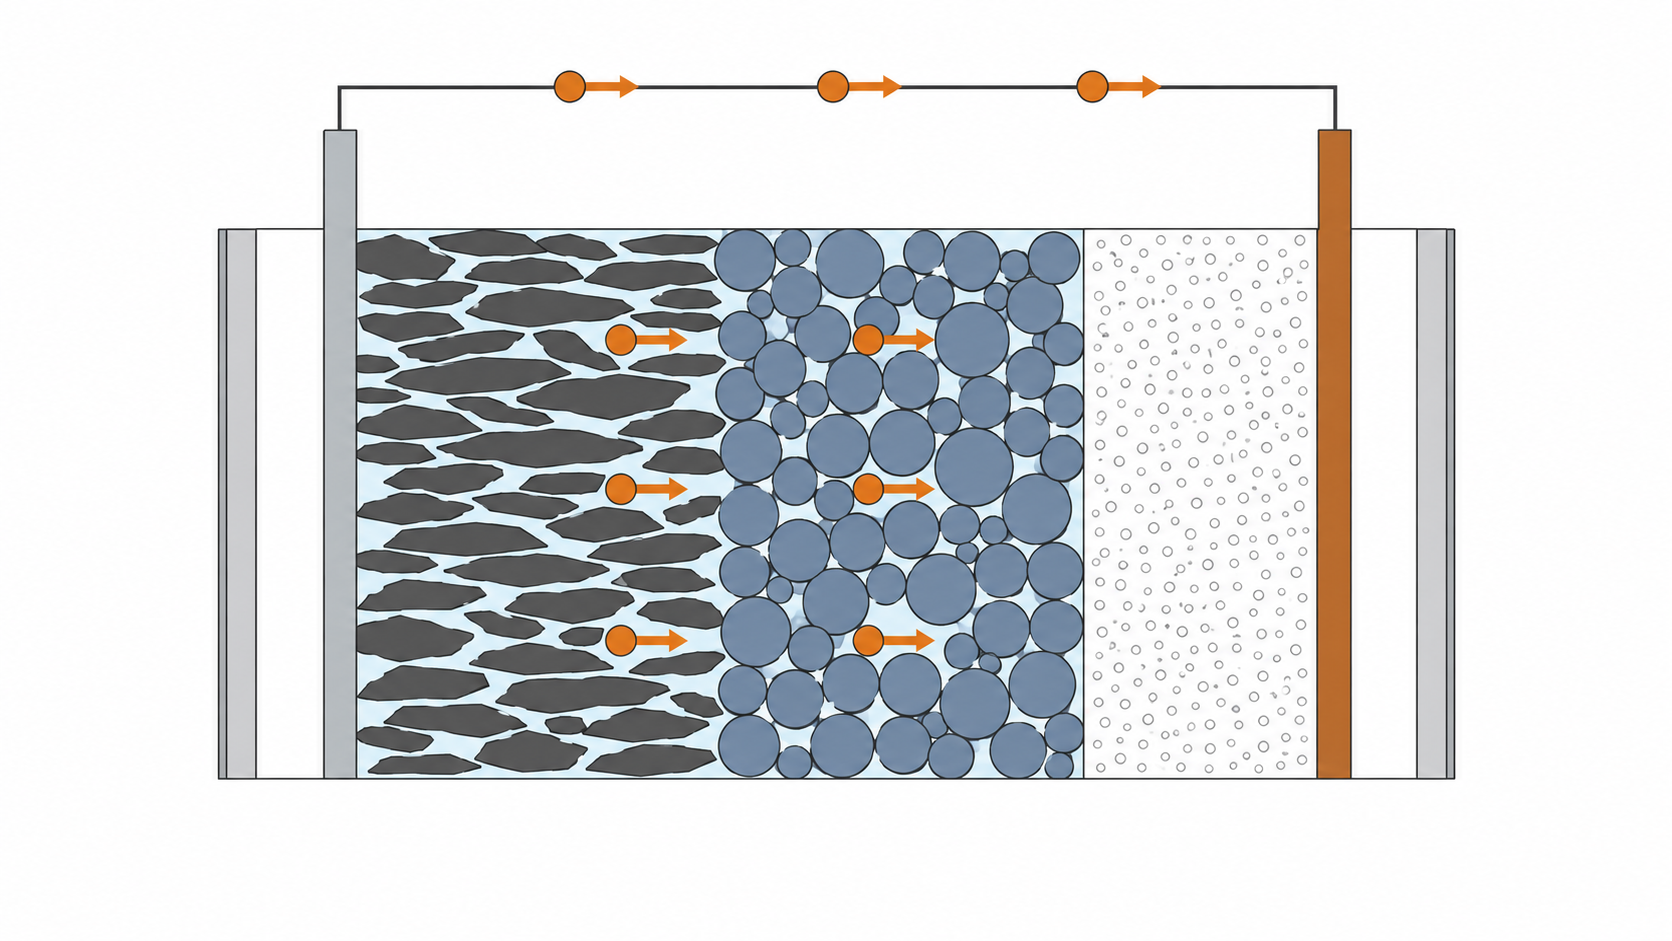
\includegraphics[width=\linewidth]{figures/ch07/ch07-07-battery-errors.png}};
  \begin{scope}[x={(img.south east)}, y={(img.north west)},
    font=\sffamily\small]
    \node[font=\bfseries] at (0.50, 1-0.02) {充电（错误示例）};
    \node[font=\scriptsize] at (0.20, 1-0.90) {铝箔};
    \node[font=\scriptsize, align=center] at (0.315, 1-0.90) {负极\\（石墨）};
    \node[font=\scriptsize, align=center] at (0.525, 1-0.90) {正极\\（如 LiCoO$_2$）};
    \node[font=\scriptsize] at (0.69, 1-0.90) {隔膜};
    \node[font=\scriptsize] at (0.76, 1-0.94) {铜箔};
    \node[font=\scriptsize, rotate=90, anchor=south] at (0.15, 1-0.20) {外壳};
    \node[font=\scriptsize] at (0.20, 1-0.11) {负极极耳};
    \node[font=\scriptsize] at (0.76, 1-0.11) {正极极耳};
    \node[font=\scriptsize\bfseries, text=white, fill=ch07err, circle, inner sep=1.5pt] at (0.20, 1-0.22) {❶};
    \node[font=\scriptsize\bfseries, text=white, fill=ch07err, circle, inner sep=1.5pt] at (0.76, 1-0.22) {❶};
    \node[font=\scriptsize\bfseries, text=white, fill=ch07err, circle, inner sep=1.5pt] at (0.42, 1-0.22) {❷};
    \node[font=\scriptsize\bfseries, text=white, fill=ch07err, circle, inner sep=1.5pt] at (0.40, 1-0.55) {❸};
    \node[font=\scriptsize\bfseries, text=white, fill=ch07err, circle, inner sep=1.5pt] at (0.50, 1-0.08) {❹};
    \node[font=\scriptsize, text=BookInk!80, anchor=north] at (0.50, 1-0.96)
      {❶–❹ 对应表~7-3 的 S2、S1、S4、S7};
  \end{scope}
\end{tikzpicture}
